\chapter{Music Representation}
\label{chap:MusicRepresentation}

This chapter explores how music is represented in this thesis. It looks at the encodings devised for the PrIMuS dataset and how they've been modified to produce our Mashcima music encoding. Then we explore how this encoding can be used for annotating datasets and how it can be extended in the future.

All the encodings explored in this chapter are made for a~model that produces a~sequence of tokens. An~encoding then defines a~specific set of tokens and describes how they map onto the musical symbols. In the context of a~neural network with a~CTC loss function, we take all the tokens of an~encoding and represent them as the individual classifier classes. How the tokens get indexed and how the blank symbol is represented is considered an~implementation detail of the neural network and is not covered in the encoding specification.

We can provide a~short overview of the terms used in this chapter:

\begin{itemize}
\item \textbf{Token} is a~single item of the output sequence produced by a~model.
\item \textbf{Vocabulary} is the set of all tokens in an~encoding.
\item \textbf{Encoding} is a~scheme for mapping musical staves onto a~sequence of tokens.
\item \textbf{Annotation} is a~specific sequence of tokens.
\end{itemize}


\section{PrIMuS Agnostic Encoding}

The PrIMuS dataset contains over 87~000~items, each with an~image of the printed staff and then multiple files describing the music in that staff. There are two standard formats, namely Music Encoding Initiative format (MEI) and the Plaine and Easie code source. Then there are two on-purpose encodings devised specifically for this dataset. These two encodings are what interests us.

\begin{figure}[h]
    \centering
    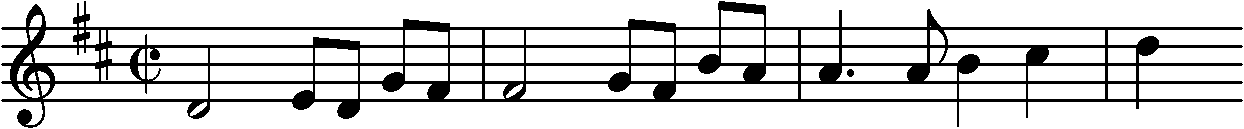
\includegraphics[width=140mm]{../img/primus-incipit}
    \verb`package_aa/000112602-1_1_1/000112602-1_1_1.png`
    \caption{An incipit from the PrIMuS dataset.}
    \label{fig4:PrimusIncipit}
\end{figure}

The first of these two encodings is the \emph{semantic encoding}. It represents what the musical symbols mean. Each symbol has a~specific pitch that relies on the cleft at the beginning of the staff. This makes the vocabulary much larger and any model using this encoding has taken the clef into account when reading the symbols. It is however much easier to transform this encoding to some well-known format like MusicXML since these formats tend to represent the meaning of a~score, not the score appearance.

\begin{figure}[h]
    \centering
    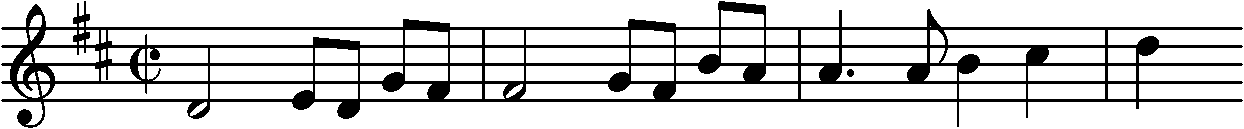
\includegraphics[width=140mm]{../img/primus-incipit}
    \verb`clef-G2`
    \quad\verb`keySignature-DM`
    \quad\verb`timeSignature-C/`
    \quad\verb`note-D4_half`
    \quad\verb`note-E4_eighth`
    \quad\verb`note-D4_eighth`
    \quad\verb`note-G4_eighth`
    \quad\verb`note-F#4_eighth`
    \quad\verb`barline`
    \quad\verb`note-F#4_half`
    \quad\verb`note-G4_eighth`
    \quad\verb`note-F#4_eighth`
    \quad\verb`note-B4_eighth`
    \quad\verb`note-A4_eighth`
    \quad\verb`barline`
    \quad\verb`note-A4_quarter.`
    \quad\verb`note-A4_eighth`
    \quad\verb`note-B4_quarter`
    \quad\verb`note-C#5_quarter`
    \quad\verb`barline`
    \quad\verb`note-D5_quarter`
    \caption{Semantic encoding of the incipit from figure~\ref{fig4:PrimusIncipit}.}
    \label{fig4:PrimusIncipitSemanticEncoded}
\end{figure}

The second encoding is the \emph{agnostic encoding}. This encoding treats the staff visually as a~specific positioning of specific symbols. It tries to capture what is in the staff visually, not what the symbols mean musically. This is comparable to a~sentence being thought of as a~sequence of letters, whereas the semantic encoding could be thought of as the specific sounds a~written sentence represents. This makes the encoding harder to convert to a~well-known format acceptable by other music software. On the other hand, this encoding is formal-enough to be easily converted to the semantic encoding, if read correctly. So this encoding lets the model do less work, therefore the model should do fewer mistakes.

\begin{figure}[h]
    \centering
    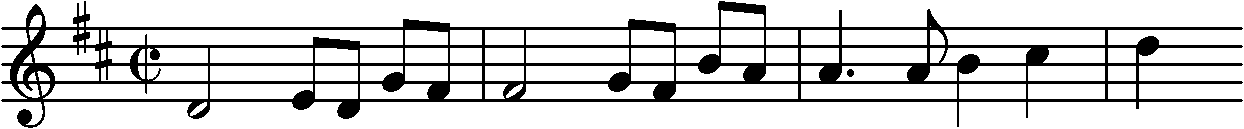
\includegraphics[width=140mm]{../img/primus-incipit}
    \verb`clef.G-L2`
    \quad\verb`accidental.sharp-L5`
    \quad\verb`accidental.sharp-S3`
    \quad\verb`metersign.C/-L3`
    \quad\verb`note.half-S0`
    \quad\verb`note.beamedRight1-L1`
    \quad\verb`note.beamedLeft1-S0`
    \quad\verb`note.beamedRight1-L2`
    \quad\verb`note.beamedLeft1-S1`
    \quad\verb`barline-L1`
    \quad\verb`note.half-S1`
    \quad\verb`note.beamedRight1-L2`
    \quad\verb`note.beamedLeft1-S1`
    \quad\verb`note.beamedRight1-L3`
    \quad\verb`note.beamedLeft1-S2`
    \quad\verb`barline-L1`
    \quad\verb`note.quarter-S2`
    \quad\verb`dot-S2`
    \quad\verb`note.eighth-S2`
    \quad\verb`note.quarter-L3`
    \quad\verb`note.quarter-S3`
    \quad\verb`barline-L1`
    \quad\verb`note.quarter-L4`
    \caption{Agnostic encoding of the incipit from figure~\ref{fig4:PrimusIncipit}.}
    \label{fig4:PrimusIncipitAgnosticEncoded}
\end{figure}

The agnostic encoding has also the advantage, that annotating an~image is not as difficult for a~human. Annotating an~image using the semantic encoding requires the annotator to know pitches for a~given key. The situation is even more complicated by key signatures. This means an~untrained non-musician has to do a~lot of thinking when annotating, which leads to many errors and slow annotation speed.

We've taken this agnostic encoding and modified it slightly to produce our Mashcima music representation.


\section{Mashcima Music Encoding}


\subsection{Notes And Pitches}

Mashcima music encoding is an~encoding that attempts to improve upon the PrIMuS agnostic encoding. In the source code, most of the logic regarding this encoding is placed inside the \texttt{app/vocabulary.py} file. Each token of this encoding represents some musical symbol.

\begin{figure}[h]
    \centering
    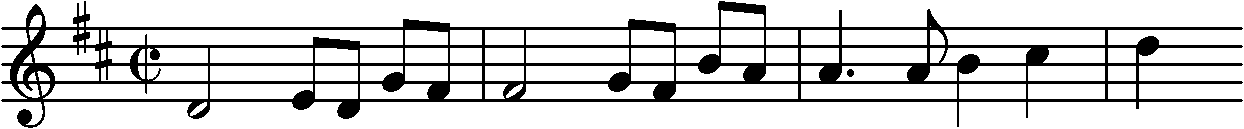
\includegraphics[width=140mm]{../img/primus-incipit}
    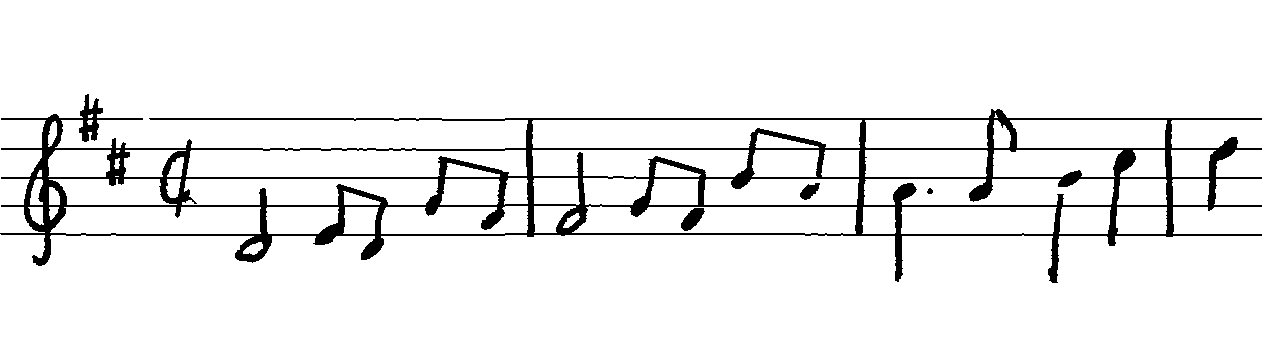
\includegraphics[width=140mm]{../img/primus-incipit-engraved}
    \verb`clef.G-2 #4 #1 time.C/ h-5 e=-4 =e-5 e=-2 =e-3 |`
    \verb`h-3 e=-2 =e-3 e=0 =e-1 | q-1 * e-1 q0 q1 | q2`
    \caption{Mashcima encoding of the incipit from figure~\ref{fig4:PrimusIncipit}.}
    \label{fig4:PrimusIncipitMashcimaEncoded}
    \medskip
    \small
    The top image is taken from the PrIMuS dataset. The bottom image is the same music engraved using our engraving system. Below that is the Mashcima encoding of the music.
\end{figure}

The first symbol we need to encode is a~note. A~note has some duration and some pitch. These two pieces of information can vary independently, so it can seem logical to represent them using two vectors. The problem is that the connectionist temporal classification can output only one vector at a~time. To solve this, we take every possible combination of note duration and pitch and create a~token for that case.

\begin{table}[h] \centering
\begin{tabular}{l@{\hspace{1.5cm}}lr}
\toprule
\textbf{Mashcima token} & \textbf{Duration} & \textbf{Pitch} \\
\midrule
\texttt{w5}  & Whole note         & 5  \\
\texttt{h0}  & Half note          & 0  \\
\texttt{q-8} & Quarter note       & -8 \\
\texttt{e-4} & Eighth note        & -4 \\
\texttt{s9}  & Sixteenth note     & 9  \\
\texttt{t12} & Thirty-second note & 12 \\
\bottomrule
\end{tabular}
\caption{All possible note durations, each with some pitch.}
\label{tab4:NoteDurations}
\end{table}

Combining duration information and pitch information into a~single token actually ends up being a~reasonable solution. That is because the concept of note duration can be extended to a~concept of symbol type in general. This is because not only notes have pitches.

The set of pitches we can choose from greatly impacts the vocabulary size. This is not a~major issue, because the vocabulary size will still remain relatively small. Currently, the vocabulary has around 550~tokens. The pitch range we choose spans from \texttt{-12} to \texttt{12} --- that is from the fourth ledger line below the staff to the fourth ledger line above the staff.

The pitch encoding is built such that it would be easy to understand for a~non-musician. In western music notation, the pitch of a~note is represented by the vertical position of that note on the staff. An~empty staff is composed of 5 staff lines. Mashcima encoding sets the middle staff line position to be zero. Going up, the first space is pitch \texttt{1} and the first line is pitch \texttt{2}. Going down, the first space is pitch \texttt{-1} and the first line is pitch \texttt{-2}.

\begin{figure}[h]
    \centering
    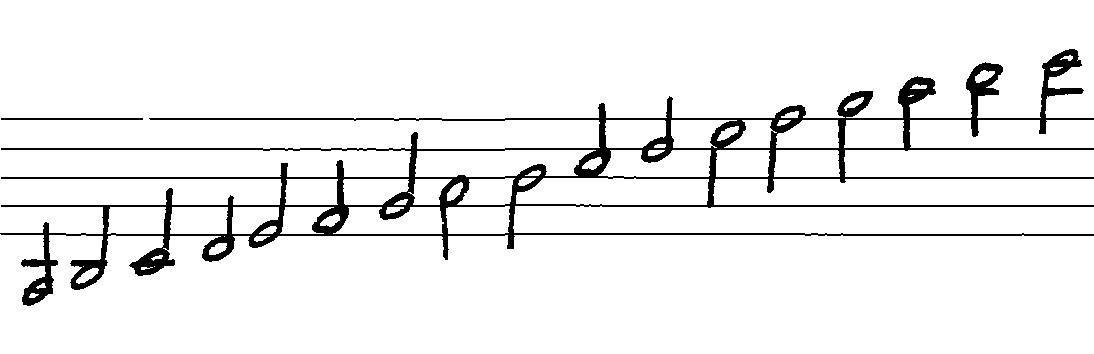
\includegraphics[width=120mm]{../img/rising-half-notes}
    \verb`h-8 h-7 h-6 h-5 h-4 h-3 h-2 h-1 h0 h1 h2 h3 h4 h5 h6 h7 h8`
    \caption{Half notes with pitches from -8 to 8.}
    \label{fig4:RisingHalfNotes}
    \medskip
    \small
    The image was engraved using Mashcima. You can see the stem orientation being randomized for pitches between -2 and 2.
\end{figure}

This pitch encoding has the advantage of being vertically symmetric, which speeds up the manual annotation process. The first ledger line above the staff is pitch \texttt{6}, and the first ledger line below is pitch \texttt{-6}. The second property this system has is that pitches placed on lines are even and pitches placed in spaces are odd.


\subsection{Rests And Barlines}

The second most common symbol is probably a~rest. A~rest has duration, just like a~note, but it has no pitch information. Its vertical position may vary, but that doesn't encode any pitch information.

\begin{table}[h] \centering
\begin{tabular}{l@{\hspace{1.5cm}}l}
\toprule
\textbf{Mashcima token} & \textbf{Duration} \\
\midrule
\texttt{lr} & Longa rest (4 measures) \\
\texttt{br} & Breve rest (2 measures) \\
\texttt{wr} & Whole rest              \\
\texttt{hr} & Half rest               \\
\texttt{qr} & Quarter rest            \\
\texttt{er} & Eighth rest             \\
\texttt{sr} & Sixteenth rest          \\
\texttt{tr} & Thirty-second rest      \\
\bottomrule
\end{tabular}
\caption{Tokens for all rests representable by the Mashcima encoding.}
\label{tab4:RestDurations}
\end{table}

You may have noticed, that that there are two extra durations --- longa and breve. Also, there is missing the sixty-fourth rest. It all has to do with the fact that not all durations are used equally frequently. I based Mashcima on the CVC-MUSCIMA and MUSCIMA++ datasets. There is no occurrence of longa or breve notes in those datasets. There are, however, occurrences of longa and breve rests. Similarly, sixty-fourth notes and rests are also not present. The vocabulary can luckily be extended to accommodate these symbols. See the section \ref{sec:RepresentationExtensibility} for more details.

Now that we have notes and rests, we can start grouping them into measures (bars). A~barline is represented by the "pipe" character (\texttt{|}). Barlines separate notes and rests into groups of the same total duration. There are many types of barlines (double barline, repeat signs) and although they are used quite often, they have not yet been implemented into the Mashcima engraving system. This is simply because we wanted to see, whether our approach even works. These special barline types can be easily added in the future.

\begin{figure}[h]
    \centering
    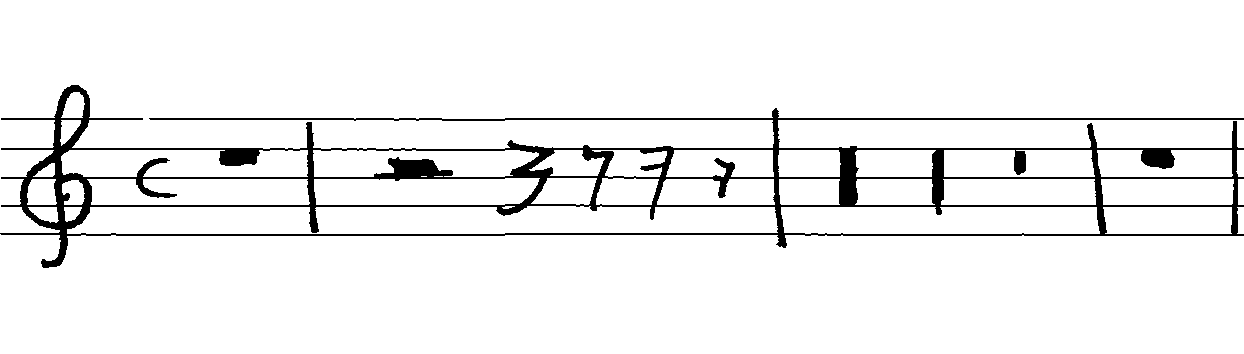
\includegraphics[width=140mm]{../img/rests-and-barlines}
    \verb`clef.G-2 time.C wr | hr qr er sr sr | lr lr br | wr |`
    \caption{Rests and barlines.}
    \label{fig4:RestsAndBarlines}
    \medskip
    \small
    The image was engraved using Mashcima. The symbols were taken from all writers and chosen randomly, therefore the two sixteenth rests look very different.
\end{figure}


\subsection{Generic Tokens}

There are some tokens that contain pitch information and some that do not. Since the pitch information is often not required when inspecting a~token sequence, it is useful to strip it away. This is why we define a~\emph{generic token} as a~version of a~token without pitch information. So for example a~generic quarter note is represented by the \texttt{q} token.

Generic tokens are not present in the vocabulary and cannot be produced by the model. They should also never appear in the gold data. They are, however, often used when analyzing a~given token sequence.

The only exception make tokens that don't contain pitch information (e.g. rests). They are considered to be their own generic token (i.e. the generic token for a~quarter rest \texttt{qr} is still just \texttt{qr}).

The vocabulary file (\texttt{app/vocabulary.py}) contains helper methods for working with pitches:

\begin{itemize}
\item \verb"to_generic(token: str) -> str"\\
Obtains generic version of a~token unless the given token is already generic.
\item \verb"get_pitch(token: str) -> Optional[int]"\\
Obtains pitch of a~token, or \texttt{None} if that token has no pitch.
\end{itemize}


\subsection{Attachments}
\label{sec:Attachments}

It's often the case, that notes are decorated with symbols that slightly modify their meaning. Since these decorating symbols are bound to the note itself, we call them \emph{attachments}. An~attachment token is simply a~token that belongs to some other non-attachment token.

Many kinds of musical symbols behave as attachments:

\begin{itemize}
\item \textbf{Accidentals} are symbols placed before a~note and they modify their pitch by a~semi-tone.
\item \textbf{Duration dots} are placed after a~note and they extend the duration of a~note.
\item \textbf{Articulation symbols} are usually placed below or above a~note and they specify how the note should be played (e.g. staccato, tenuto, accent).
\item \textbf{Other symbols}, like a~tuplet number, fermata, trill, etc.
\item \textbf{Artificial tokens}, that we've added to encode specific time-spanning symbols. See the section \ref{sec:RepresentationSlurs} on slurs to learn more.
\end{itemize}

You can see, that the term \emph{attachment} is not a~musical term and it describes more how a~symbol is represented, not what a~symbol means.

All of these attachments lack pitch information since the pitch is stored in the note token. The only exception here is accidentals. Accidentals are special because they need not be attached to a~note. They can be standalone in a~key signature. This means that they need pitch information. This creates some redundancy in the encoding; when a~note has an~accidental, they both should have the same pitch. This condition is not ideal, because it may cause the model to make unnecessary errors. It is however better than having different tokens for standalone accidentals and attached accidentals.

\begin{table}[h] \centering
\begin{tabular}{l@{\hspace{1.5cm}}lr}
\toprule
\textbf{Mashcima token} & \textbf{Accidental} & \textbf{Pitch} \\
\midrule
\verb"#5"  & Sharp        & 5  \\
\verb"b4"  & Flat         & 4  \\
\verb"N-4" & Natural      & -4 \\
\verb"x8"  & Double sharp & 8  \\
\verb"bb0" & Double flat  & 0  \\
\bottomrule
\end{tabular}
\caption{All accidentals, each with some pitch.}
\label{tab4:Accidentals}
\end{table}

Attachments come in two kinds:

\begin{itemize}
\item \textbf{Before attachments} are placed before the target token
\item \textbf{After attachments} are placed after the target token
\end{itemize}

By placement, we mean placement in the token sequence. It may not correspond to the visual order of the symbols. The rule of thumb here is that tokens are ordered from left to right and from top to bottom. The problem is that some symbols may be both above and below a~note, depending on the note pitch. Therefore we didn't make this into a~strict rule and instead devised a~specific ordering of the attachments:

\begin{table}[h] \centering
\begin{tabular}{l@{\hspace{1.5cm}}l}
\toprule
\textbf{Before attachments} & \textbf{Meaning} \\
\midrule
\verb")"          & Slur end      \\
\verb"fermata"    & Fermata       \\
\verb"trill +"    & Trill         \\
\verb"tuplet.3"   & Tuplet number \\
\verb"# b N x bb" & Accidentals   \\
\bottomrule
\end{tabular}
\caption{Before attachments, properly ordered.}
\label{tab4:BeforeAttachments}
\end{table}

\begin{table}[h] \centering
\begin{tabular}{l@{\hspace{1.5cm}}l}
\toprule
\textbf{After attachments} & \textbf{Meaning} \\
\midrule
\verb"."         & Staccato      \\
\verb"_"         & Tenuto        \\
\verb">"         & Accent        \\
\verb"^"         & Marcato       \\
\verb"* **"      & Duration dots \\
\verb"("         & Slur start    \\
\bottomrule
\end{tabular}
\caption{After attachments, properly ordered.}
\label{tab4:AfterAttachments}
\end{table}

Here are a~few notes regarding the ordering:

\begin{itemize}
\item Slurs are always the first/last attachment.
\item Some tokens are mutually exclusive, so they are placed on the same level.
\item There are many ornaments and this list is not exhaustive. It is meant to be extended in the future.
\item Not all symbols here can be engraved by Mashcima.
\item There can be many more tuplet numbers, only triplets are currently present.
\end{itemize}


\subsection{Slurs}
\label{sec:RepresentationSlurs}

Slurs and ties are one of the first symbols that make OMR complicated. A~slur is a~curved line going from one notehead to another. Notes that are under a~slur should be played blended without explicit note beginnings. A~tie looks exactly like a~slur, just the two notes it joins have the same pitch. This means the notes should be played as one long note. So the difference is only semantic, we will consider ties to be just like slurs.

\begin{figure}[h]
    \centering
    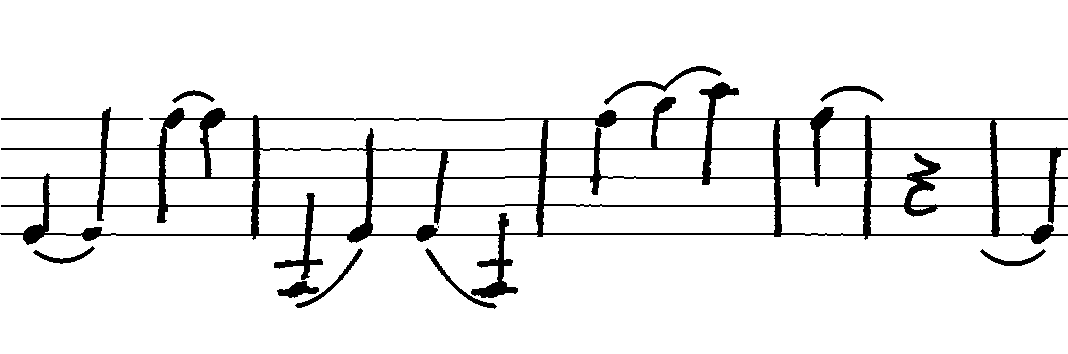
\includegraphics[width=140mm]{../img/slurs}
    \verb`q-4 ( ) q-4 q4 ( ) q4 | q-8 ( ) q-4 q-4 ( ) q-8 |`
    \verb`q4 ( ) q5 ( ) q6 | q4 ( ) | qr | ( ) q-4`
    \caption{Ties and slurs.}
    \label{fig4:Slurs}
    \medskip
    \small
    Image of various slur situations, engraved using Mashcima. The first two slurs are actually ties. One note is simultaneously a slur ending and a slur beginning. Two slurs end on a barline.
\end{figure}

Mashcima encoding does not represent slurs explicitly, but it represents their beginnings and ends. This is accomplished by two attachment tokens, \verb`(` and \verb`)`. The problem it creates is that sometimes it's impossible to pair beginnings and ends properly. Therefore we can only annotate staves that don't contain nested slurs.

Slurs can also span from one staff to the next. When this happens, the slur ends at a~barline. Therefore a~barline can also act as a~token, on which a~slur can start or end.


\subsection{Beams}

Beamed notes pose similar problems as slurs, but they obey some additional constraints that make them easier to deal with. Beams are encoded from the perspective of a~single note within the beamed group. The duration of this note depends only on the number of beams passing through its stem. We just need to distinguish the note from its flag variant, therefore we add some information regarding the beam presence. The last problem is, that having a~couple of beamed notes in a~row does not tell us about the way the beams are grouped. Therefore we modify the beam presence information into two parts --- beam ending and beam starting.

Therefore for a~given note duration, we get three tokens, that represent all the possible beam situations:

\begin{figure}[h]
    \centering
    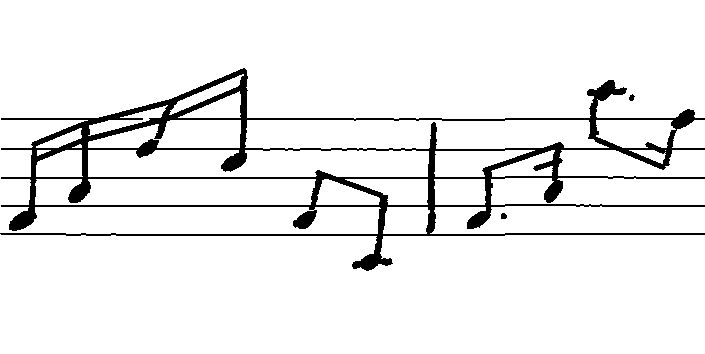
\includegraphics[width=100mm]{../img/beams}
    \verb`s=-3 =s=-1 =s=2 =s1 e=-3 =e-6 | e=-3 * =s-1 e=6 * =s4`
    \caption{Beamed notes use the \texttt{=} sign in token names.}
    \label{fig4:Beams}
\end{figure}

This, however, lets us create annotations that make no sense. We can create un-finished and non-started beams. For this reason, there is the \verb`repair_`\allowbreak\verb`annotation` function in the file \verb`app/vocabulary.py` that can repair such situations or validate the correctness of an~annotation.


\subsection{Key Signatures and Time Signatures}

A key signature is just a~group of many accidentals, typically at the beginning of a~staff. These accidentals are not attached to any note, so they have special handling in the source code. They are not a~problem from the annotation point of view.

A time signature is either a~symbol $C$ or a~pair of two numbers on top of each other. The standalone $C$ symbol can be represented easily using the \verb`time.C` token. A~pair of numbers is represented by two tokens, e.g. \verb`time.3 time.4`. Numbers have to be paired. Non-paired time number is considered an~invalid annotation.

\begin{figure}[h]
    \centering
    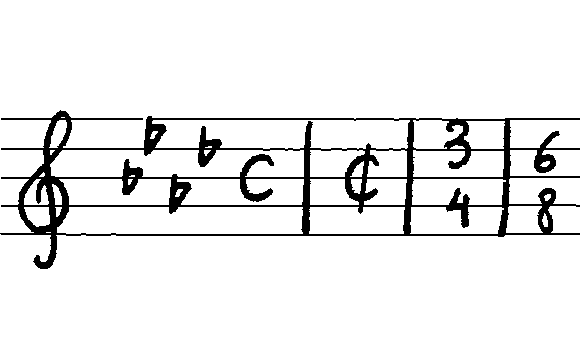
\includegraphics[width=100mm]{../img/key-and-time-signatures}
    \verb`clef.G-2 b0 b3 b-1 b2 time.C | time.C/ |`
    \verb`time.3 time.4 | time.6 time.8`
    \caption{Examples of a key signature and various time signatures.}
    \label{fig4:KeyAndTimeSignatures}
\end{figure}

Time signature numbers are also treated specially since they always come in pairs.


\subsection{Clefs and Repeats}

Clefs are encoded similarly to rests, with the only difference of having a~pitch associated. Not all pitches are allowed, though. There are three types of clefs (G, C, F). Each of these clefs has a~set of pitches it can have.

\begin{figure}[h]
    \centering
    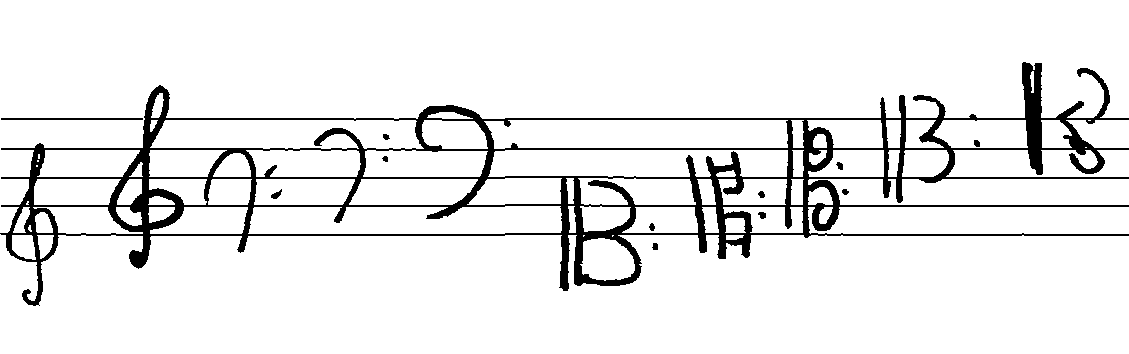
\includegraphics[width=120mm]{../img/clefs}
    \verb`clef.G-4 clef.G-2 clef.F0 clef.F2 clef.F3`
    \verb`clef.C-4 clef.C-2 clef.C0 clef.C2 clef.C4`
    \caption{Various clefs by various writers.}
    \label{fig4:Clefs}
\end{figure}

There are special barlines that mark a~part of music to be repeated. These barlines cannot be engraved yet, but they do have corresponding tokens in the encoding: \verb`:|`, \verb`|:`, \verb`:|:`.


\section{Differences to PrIMuS}

Mashcima encoding is very similar to the agnostic PrIMuS encoding, but there are some deliberate changes introduced. Mashcima encoding has on purpose shorter token names. This aims to aid readability when manually annotating. The goal is to fit one staff of tokens onto the screen. Common tokens, like quarter notes (\verb`q5`), are also quick to type. We also decided to use characters that look like the musical symbols they encode (sharps \verb`#5`, flats \verb`b5`, barlines \verb`|`).

The pitch is also encoded differently. In PrIMuS agnostic encoding, every token has a~pitch --- even a~barline. The pitch might not be useful, but it's present, to simplify working with the encoding. We decided to leave some tokens without pitch information. That complicates the code but makes the annotation more user-friendly.

Also, the specific pitch values are different. PrIMuS indexes lines and spaces separately and line zero is the first ledger line below the staff. We tried to improve on this by putting the line zero at the center of the staff. This makes the pitch values vertically symmetric. We also removed the separation of lines and spaces and we use just an~integer value. That simplifies the code that deals with pitch information. This integer value is then odd in spaces and even on lines.


\section{Extensibility}
\label{sec:RepresentationExtensibility}

Because the CVC-MUSCIMA dataset contains such a~wide range of symbols, we didn't want to create an~encoding that would capture every possible symbol in the dataset. Most of these unusual symbols are present in only a~few places and adding them to the encoding would make everything much more complicated, for little to no return. Therefore the Mashcima encoding contains the \verb`?`~token. This token should be placed into gold data whenever we encounter a~symbol (or a~group of symbols) that cannot be represented by our encoding. This \verb`?`~token acts as a~marker, that we cannot fully represent a~specific place in the staff. It can then be used to filter out such bars or just to find such places if the encoding was ever extended in the future.

As mentioned in previous sections, there are missing some note and rest durations. These can be easily added when needed. These new tokens would follow the rules that are imposed onto all the current notes and rests.

Similarly, many symbols are not present in the encoding but could be easily added. Dynamics cannot be encoded right now. They are ignored as if they weren't present at all. They could be added as \emph{after attachments}. The same applies to additional tuplets or similar ornaments.

Grace notes are special. They look like little notes, they do not affect the rhythm and are considered an~ornament attached to another note. PrIMuS agnostic encoding can represent them but at the expense of adding a~lot of additional tokens. We decided not to bloat our vocabulary with symbols that aren't very abundant in the CVC-MUSCIMA dataset. They are present in a~few places in the evaluation dataset and are represented by the \verb`?` token.

A chord is two or more notes played simultaneously. Currently, there is no way of encoding simultaneous notes. Since chords usually share a~stem, they could maybe be represented via after attachments. Maybe if we encoded the top-most note of a~chord as a~regular note and then added one "notehead" token for every remaining note, we could represent a~chord. But there are problems with having multiple accidentals. Either way, it would be interesting to explore in some future work.

Text (like lyrics and tempo) is also ignored. It is not encoded by even the \verb`?`~token.
